\section{Durchführung}

\subsection{Kalibriermessungen}
    \subsubsection{Messung einer Quelle bekannter Aktivität bei mittiger Quellposition}
       Zunächst haben wir eine Quelle in mittigem Abstand zu den beiden Detektoren vermessen. Die Quelle hatte am 29.10.2015 eine Aktivitiät $A = 1,02 MBq$.\\
       \vspace{2mm}
       \minipanf 
                  \makebox[\textwidth]{\scalebox{0.5}{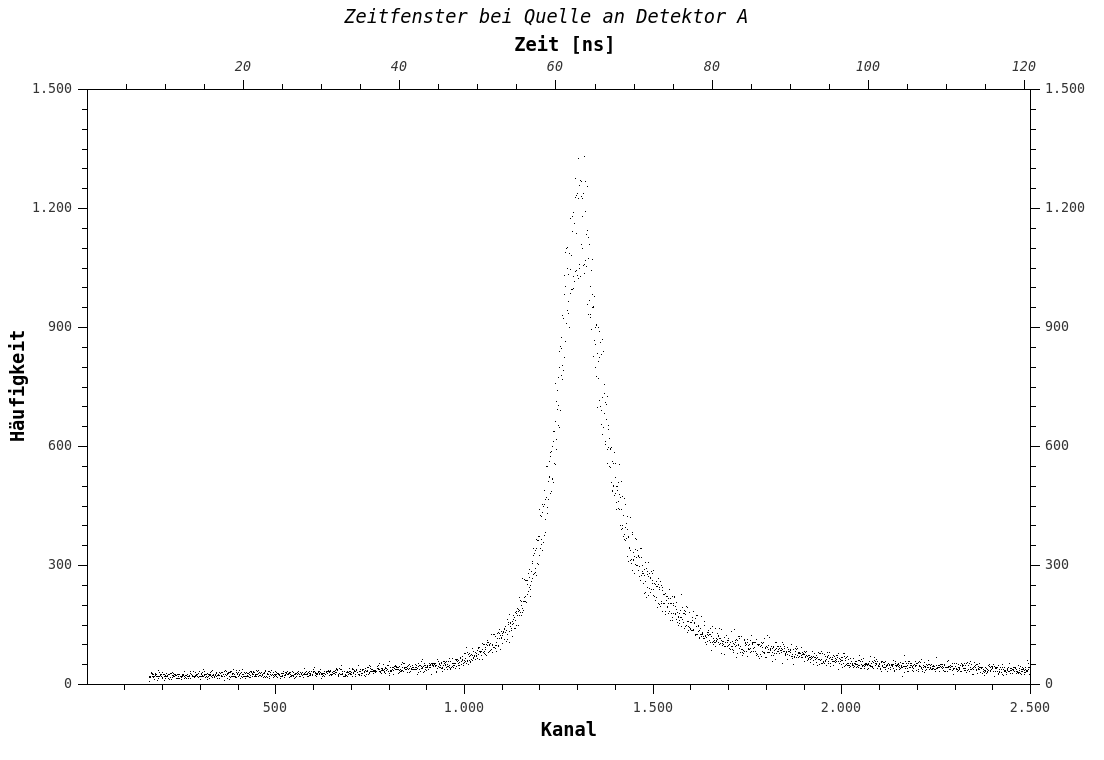
\includegraphics{../2015_10_29/qtiplots/notfallbilder/T_A_dia.png}}}
                  \label{dfd:T_A}
       \minipend
       \minipanf 
       \vspace{3mm}
       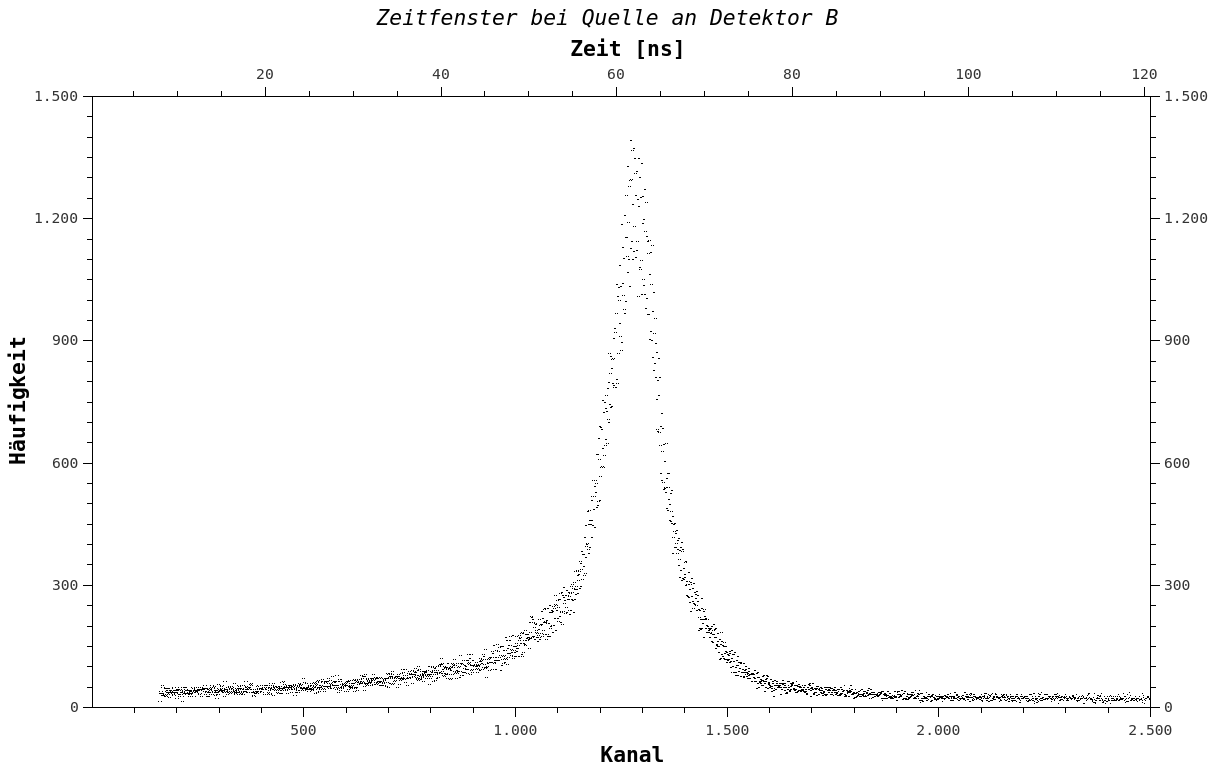
\includegraphics{../2015_10_29/qtiplots/notfallbilder/T_B_dia.png}
       \label{dfd:T_B}
       \minipend       

    \subsubsection{Messung bei Positionen direkt an den Detektoren}

        
